\documentclass[../main.tex]{subfiles}

\chapter{Spoof simulation tests}
When a GPS receiver is spoofed, its solved position or time (or both) might change. The result depends on the technique used to spoof. By moving a GPS receiver, one can simulate a spoofing attack since the location most certainly will change. It might also affect the time solved (but why? Figure this out). We also covered the antennas with aluminium foil to simulate a loss of signal.

\section{Data acquisition}\label{data_aquisition}
In order to create an accurate clock-model of the atomic clock, it was necessary to log data from it while it was running in a disciplined mode. In the disciplined mode, the atomic clock will correct it's frequency based on either a 1 PPS (Pulse per second) signal or a 10 MHz signal as discussed earlier under section (\ref{csac_com}) A similar approach was used in order to collect GPS data. Data from two u-blox NEO-M8T was gathered over the same time period as the data gathered from the atomic clock. By gathering the data over the same period, it was possible to detect any correlation between the time solved by the GPS receivers and any frequency adjustments done by the atomic clock. It also provided valuable data that could be used to tune the filters in the atomic clock controller. The data gathering was done by simple Python scripts (appendix \ref{CL} and \ref{GL}) running on a computer connected to the GPS receivers and the atomic clock. Figure (\ref{CLS}) shows a block diagram of the setup.

\section{Setup}
\begin{figure}
\centering
  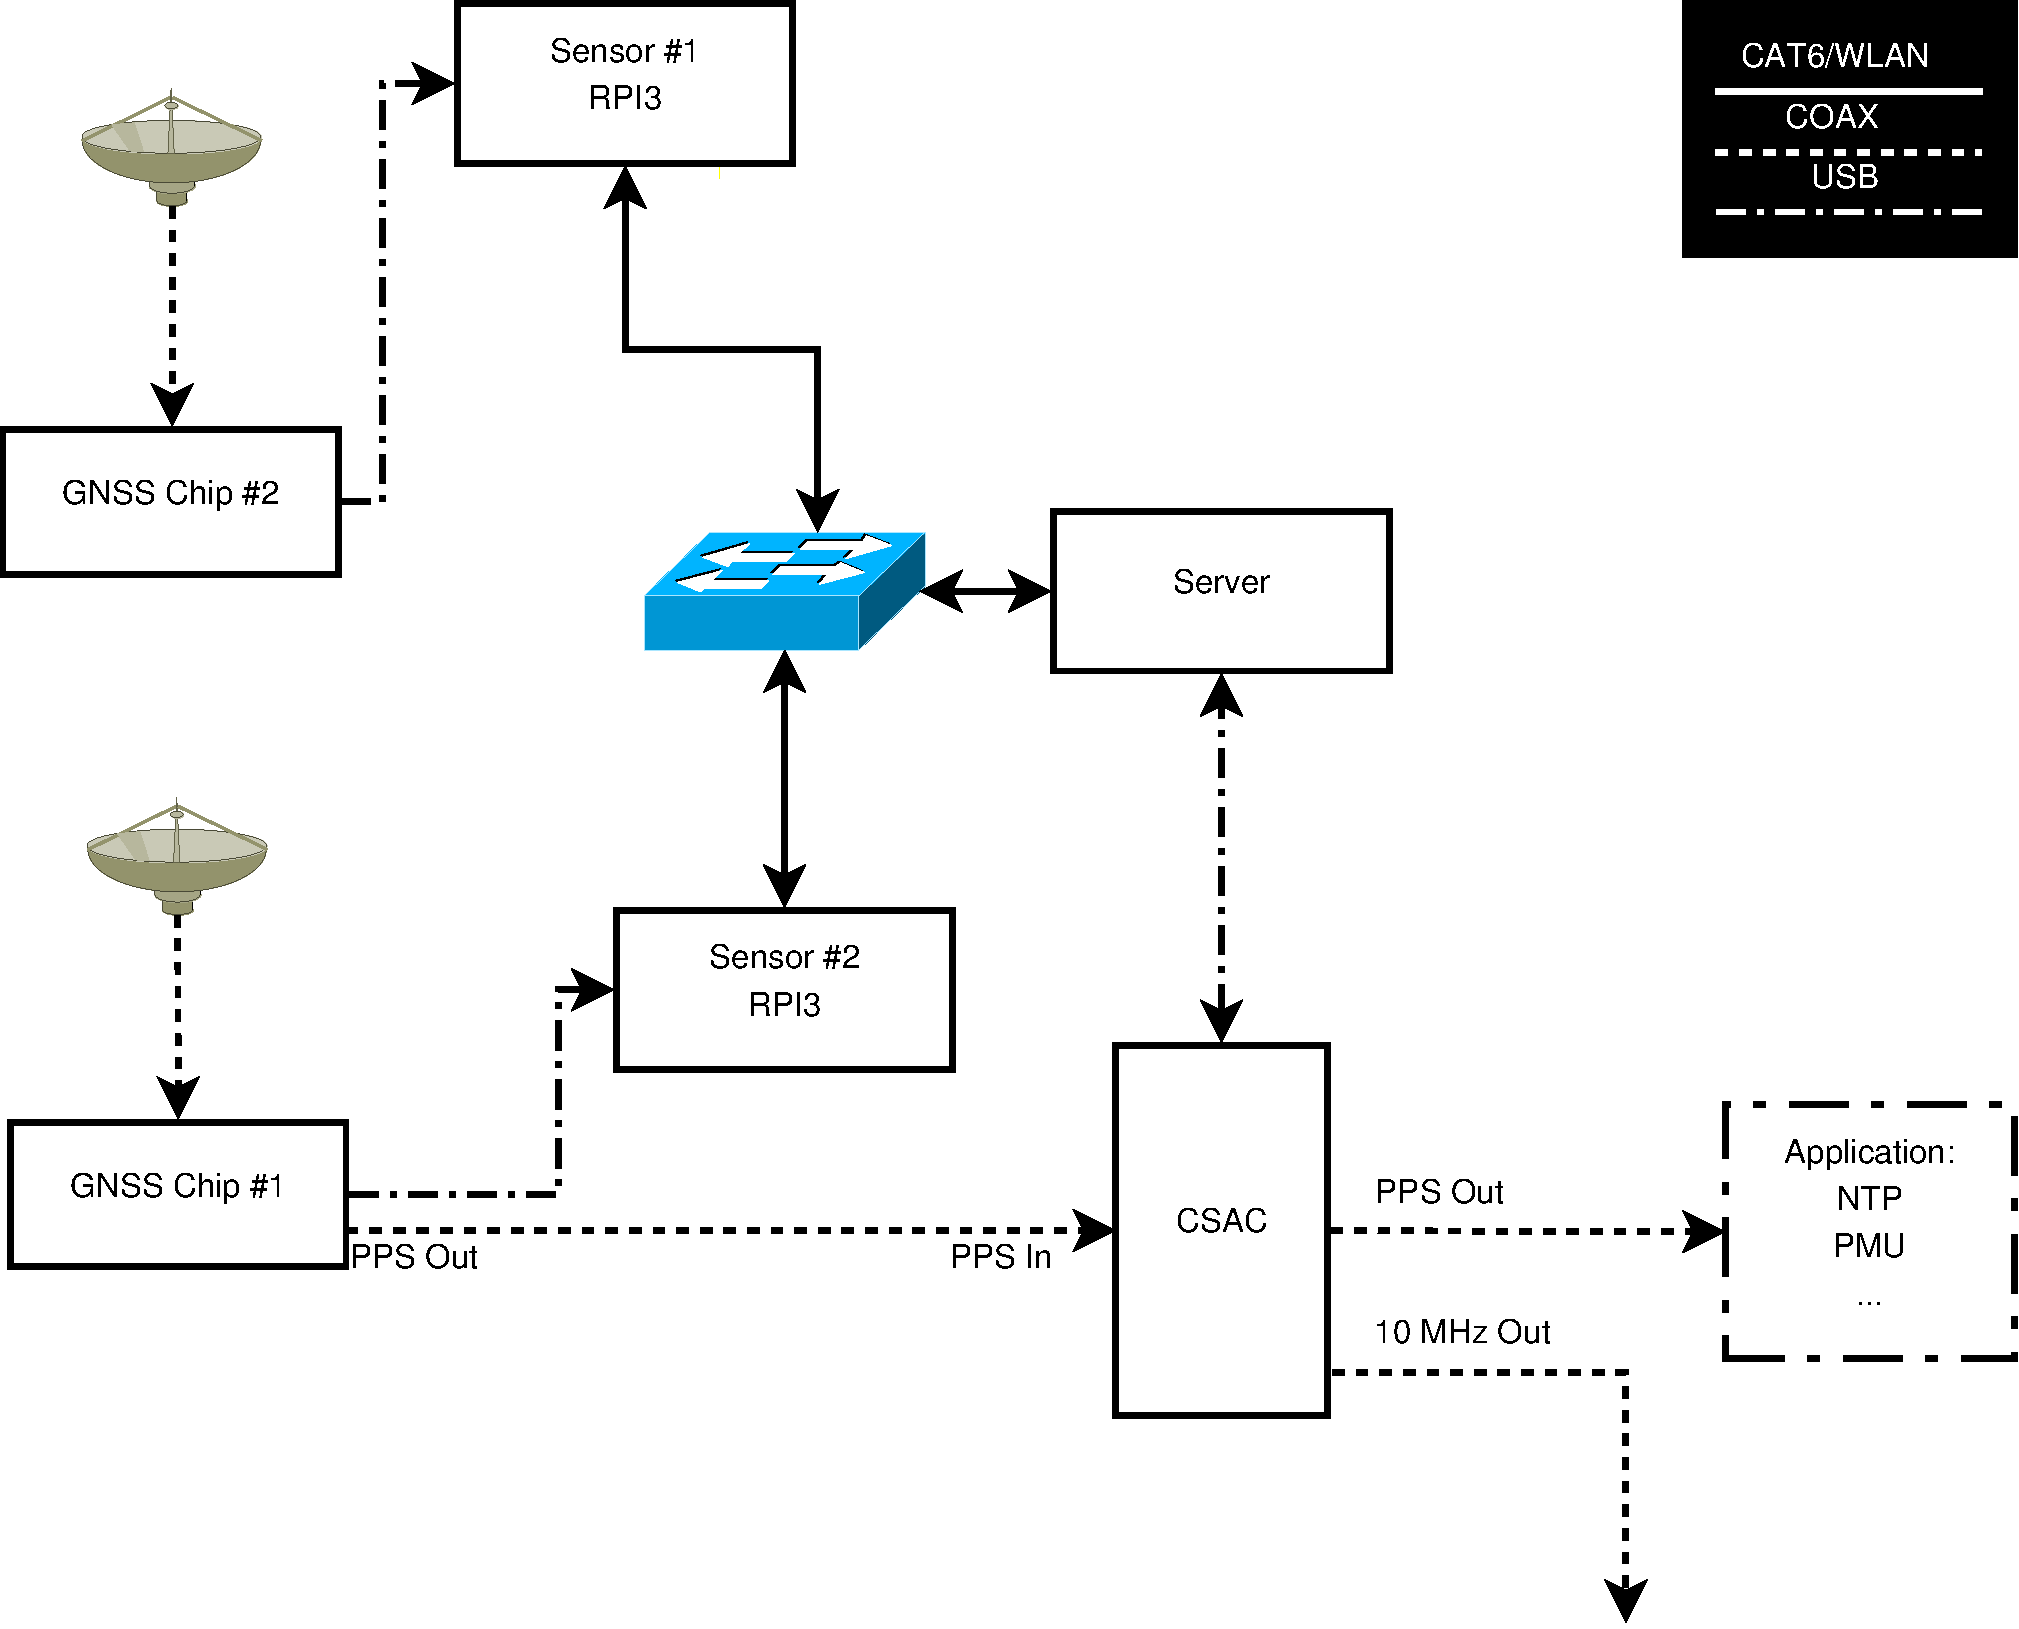
\includegraphics[scale=0.31]{server_layout.pdf}
   \caption[atomic clock controller implementation block diagram]{A block diagram showing the tested implementation.}
   \label{ibd}
\end{figure}

Figure \ref{ibd} shows how the Server, Sensors and atomic clock were physically set up. In order to assure good GPS satellite geometry, the antennas were placed at the roof of Justervesenets main office at Kjeller. Antenna 1 was placed at a railing about a 1 meter above the ground, antenna 2 was placed at ground level. Antenna 1 was connected to GPS receiver 1 which in turn was connected to Sensor 1. It's the same deal with antenna 2 which was connected to GPS receiver 2 which in turn was connected to Sensor 2. The distance between the two antennas was about 35 meters. The antenna connected to Sensor 1 did not utilize the full length of it's cable. This is because it proved challenging to find a place where the antenna could be placed in stable position, yet use the full length of the cable. The Sensors and the Server were connected to LAN through a Gigabit ethernet switch. The Server was configured to log telemetry received from the atomic clock and the Clients were configured to log all NMEA data received from the GPS receivers. The GPS receiver connected to antenna South is used to supply the atomic clock with a 1 PPS signal. Because the atomic clock model needs live data over time to mature, the system was started Friday 7. October 2016 and the test was performed Monday 10. October 2016. Figure \ref{msd} is a block diagram showing how the measuring setup was physically configured. Figure \ref{lab_setup_photo} is a photograph of the measuring setup. Not shown in the photo, is the source of the 10 MHz signal used a reference. This signal was carried by cable from the time laboratory at the second floor.

\begin{figure}[!htb]
\centering
  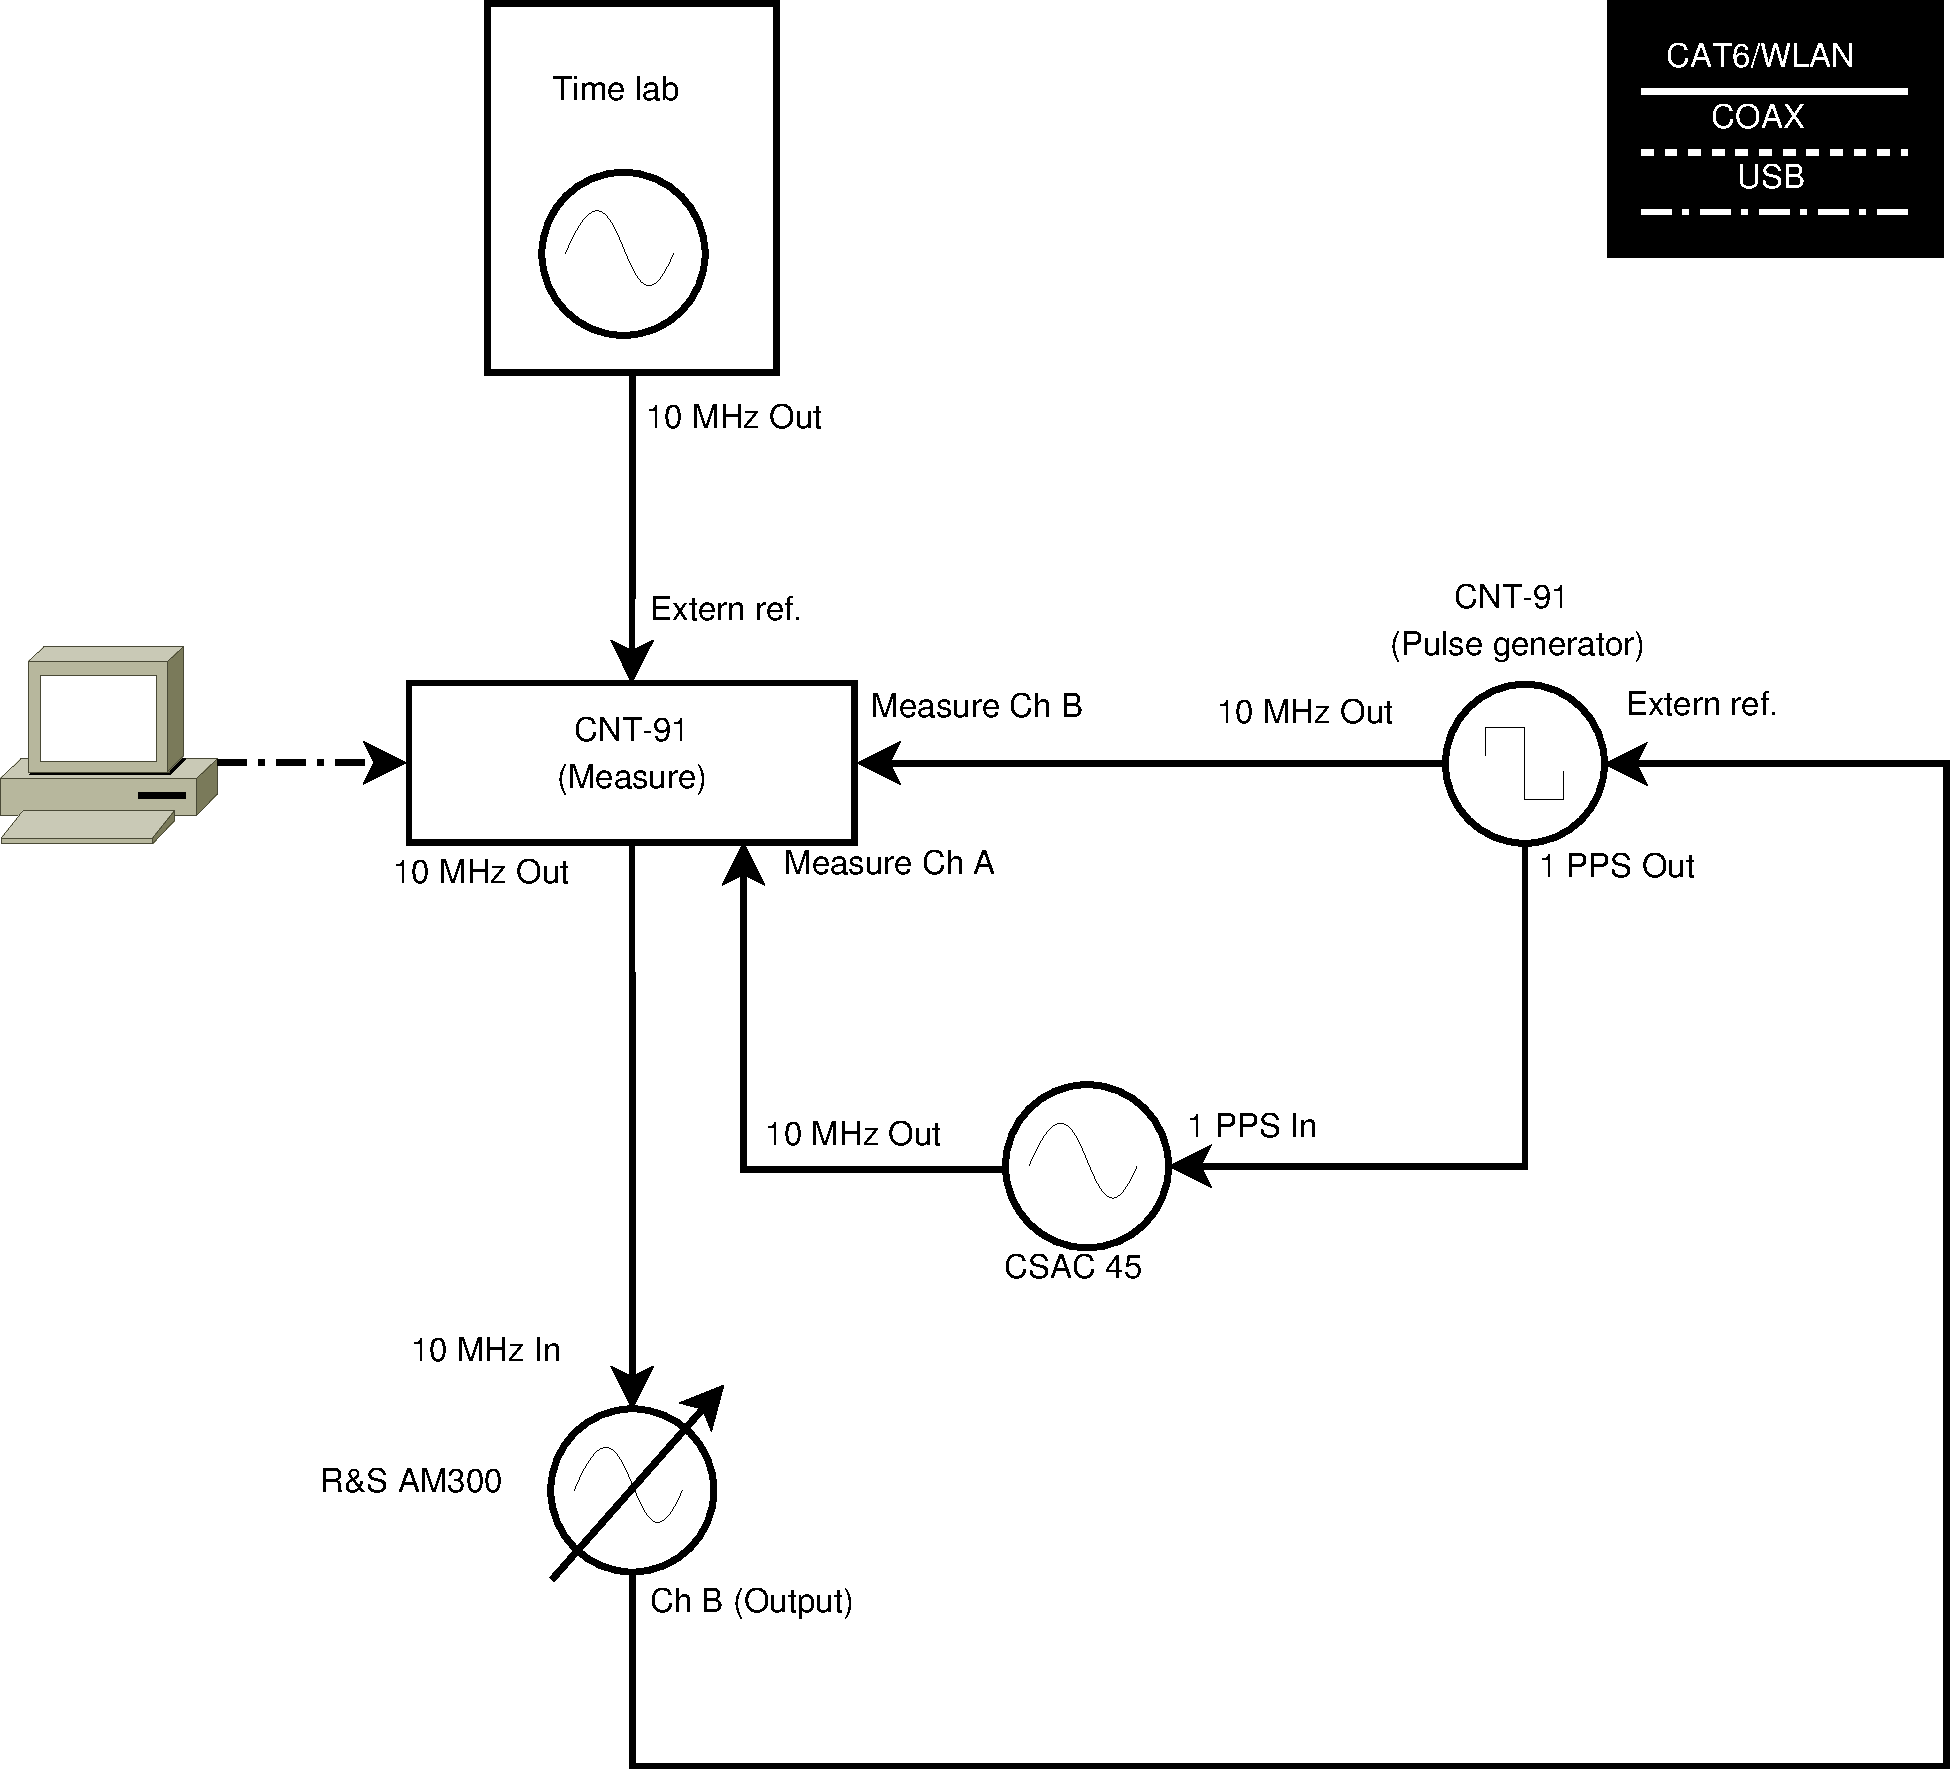
\includegraphics[scale=0.31]{measure_setup.pdf}
   \caption[Measurement setup]{Block diagram showing the setup of the measurement equipment}
   \label{msd}
\end{figure}

\section{Test 1}
\subsection{Goal of test}
The goal with this test was to use the Sensor Server system to detect a simulated spoofing attack. By moving the antennas, the KRL filter should be triggered as the solved longitude, altitude, latitude and speed should change. See \ref{kvsrlf} for more about the KRL filter. The clock model based filters might also trigger. See \ref{csac_filters}. The result would be observable by analyzing the log files produced by the Server and Clients and the data collected by the measuring setup.

\subsection{Description}\label{test1_description}
The following is a step by step description of how the test was conducted. The time in the brackets was obtained from a wristwatch. It is written in the normal format as well as number of seconds after 10:48. This is because the data used to draw the graphs, started at 10:48 but uses seconds in the X axis. Comparison is therefore easier. It is important to note that nor the resolution or accuracy was of any notable concern when writing down the time. The time was mainly noted to make it easier to find any correlation between the steps taken and patterns found in the log files. 

\begin{itemize}
  \item\relax 10:58 - 600: Moved antenna 1 approximately 15 meters to the south.
  \item\relax 11:03 - 900: Moved antenna 1 back to original location.
  \item\relax 11:07 - 1140: Moved antenna 2 approximately 15 meters to the north.
  \item\relax 11:12 - 1440: Moved antenna 2 back to original location.
  \item\relax 11:14 - 1560: Waved antenna 1 around horizontally in a half circle motion at an increasing tempo.
  \item\relax 11:18 - 1800: Waved antenna 2 around horizontally in a half circle motion at an increasing tempo.
  \item\relax 11:20 - 1920: Covered antenna 1 with aluminium foil.
  \item\relax 11:25 - 2220: Covered antenna 2 with aluminium foil.
  \item\relax 11:28 - 2400: Removed foil from antenna 1.
  \item\relax 11:33 - 2700: Removed foil from antenna 2.
\end{itemize}
\newpage

\begin{wrapfigure}{r}{0.40\textwidth}
  \centering
  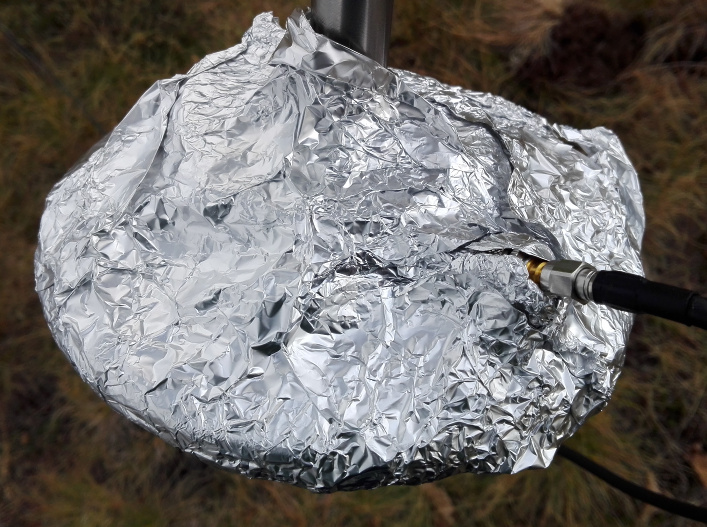
\includegraphics[width=0.40\textwidth]{antenna_foil_cover.jpg}
  \caption[Antenna covered in aluminium foil]
   {Antenna covered in aluminium foil to simulate a jamming attack.}
\end{wrapfigure} 

Step 1 and 2 were designed to trigger the KRL filter, especially the check of solved latitude, longitude and altitude but also the speed, against known values. Step 5 and 6 was also designed to trigger the KRL filter, but more specifically the checking of solved speed. Step 7 and 8 was to designed to reveal what would happen with the both the KRL and the CM filter during a jamming attack as it was believed that covering the antennas with aluminium foil would block all signals out.

\subsection{Observations}\label{test1_observations}
\subsubsection{Sensor Server logs}
By reviewing the log produced by the Sensor Server, the following was observed:

\begin{itemize}
  \item No false positives, the filters were not triggered before the test started.
  \item The KRL filter was triggered by Sensor 1 at 10:59:19 and cleared at 11:04:35.
  \begin{lstlisting}
    [10/10/16 - 10:59:17] [ ALARM ] Sensor 1 triggered KRL filter!
    ...
    [10/10/16 - 11:04:35] [ ALARM ] Sensor 1 cleared KRL filter!
  \end{lstlisting}
  \item The KRL filter was triggered again at 11:08:27, but this time by Sensor 2. The alarm was cleared at 11:13:43.
    \begin{lstlisting}
    [10/10/16 - 11:08:27] [ ALARM ] Sensor 2 triggered KRL filter!
    ...
    [10/10/16 - 11:13:43] [ ALARM ] Sensor 2 cleared KRL filter!
  \end{lstlisting}
  \item Once again, 11:22:03 the KRL filter was triggered by Sensor 1 and was not cleared until 11:29:21
     \begin{lstlisting}
    [10/10/16 - 11:22:03] [ ALARM ] Sensor 1 triggered KRL filter!
    ...
    [10/10/16 - 11:29:21] [ ALARM ] Sensor 1 cleared KRL filter!
  \end{lstlisting} 
  \item At 11:27.05, it was the CM filter using the clock model that triggered. It stopped triggering 11:27:33. Sensor 2 also triggered the KRL filter 11:27:31 and cleared at 11:34:16.
    \begin{lstlisting}
    [10/10/16 - 11:27:05] [ ALARM ] Steer > limit!
    ...
    [10/10/16 - 11:27:31] [ ALARM ] Sensor 2 triggered KRL filter!
    ...
    [10/10/16 - 11:27:33] [ ALARM ] Steer > limit!
  \end{lstlisting} 
  \item The last 6 seconds, Sensor 2 triggered KRL filter and the clock model based filter was triggered at multiple occasions.
  \begin{lstlisting}
    [10/10/16 - 11:34:15] [ ALARM ] Sensor 2 triggered KRL filter!
    [10/10/16 - 11:34:16] [ ALARM ] Sensor 2 cleared KRL filter!
    [10/10/16 - 11:34:17] [ ALARM ] Sensor 2 triggered KRL filter!
    [10/10/16 - 11:34:18] [ ALARM ] Sensor 2 triggered KRL filter!
    [10/10/16 - 11:34:19] [ ALARM ] Sensor 2 triggered KRL filter!
    [10/10/16 - 11:34:19] [ ALARM ] Steer > limit!
    [10/10/16 - 11:34:20] [ ALARM ] Steer > limit!
    [10/10/16 - 11:34:20] [ ALARM ] Sensor 2 cleared KRL filter!
    [10/10/16 - 11:34:21] [ ALARM ] Steer > limit!
  \end{lstlisting} 
\end{itemize}

\subsubsection{GPS data}\label{gpsdata_test1}
The following figures are plots of the GPS data (NMEA) that was logged by the Sensors during test 1. Figure \ref{sensor1_alt} shows the altitude in meters for Sensor 1. The only thing that stands out in the plot, is when the antenna is covered in aluminium foil as show at around the 2000 second mark. At this point, the receiver is no longer able to solve a position thus generating valid but empty fields in the data. This creates a deep chasm in the plot. Because both receivers' antennas were covered in foil, all the plots share this trait. Figure \ref{sensor2_alt} shows the altitude in meters for Sensor 2. When compared with the altitude plot for Sensor 1 \ref{sensor1_alt}, Sensor 1 seems to correlate better. It is a puzzle why the Sensor 2 reported to have been moved 7 meters down, which it clearly was not. When examining figure \ref{sensor1_lat} and \ref{sensor2_lat}, showing the latitude for Sensor 1 and 2 (in that order), one can clearly see that Sensor 1 was moved to the south and Sensor 2 was moved to the north. One might also notice that Sensor 2 traveled further. The difference in travel is because Sensor 1's antenna did not utilize the full length of cable. Figure \ref{sensor1_long} and \ref{sensor2_long} shows a plot for the solved longitude for Sensor 1 and Sensor 2. When examining figure \ref{sensor1_long}, it seems as if the antenna was never moved. This is because the building the antenna was placed on, is position in a north to south line and the receiver was moved along with the roof. The antenna connected to Sensor 2 was not moved in straight line because the cable got caught in vegetation. The last two figures, figure \ref{sensor1_speed} and figure \ref{sensor2_speed} shows the speed solved by Sensor 1 and Sensor 2. They both correlate well with when the antennas were moved, however, the antenna connected to sensor 2 seems to be a little bit more sensitive than the on connected to Sensor

\begin{figure}
  \centering
  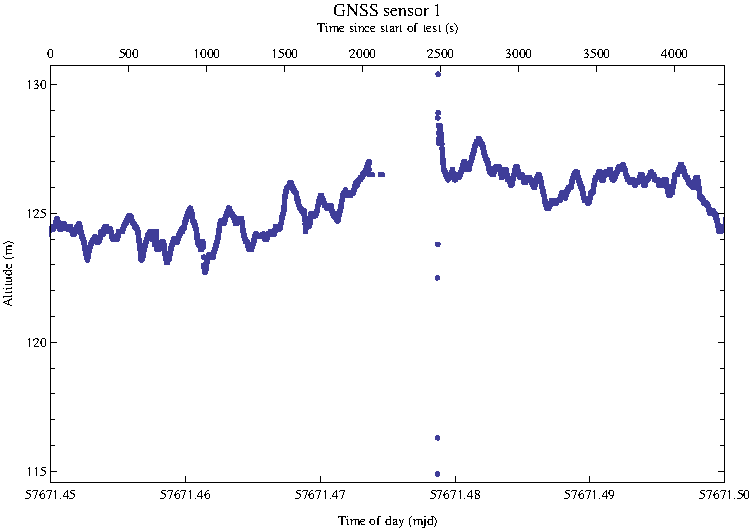
\includegraphics[width=1\textwidth]{gnssAlt1.pdf}
  \caption{The figure shows the solved altitude of the GPS receiver connected to Sensor 1, during test 1}
  \label{sensor1_alt}
\end{figure} 

\begin{figure}
  \centering
  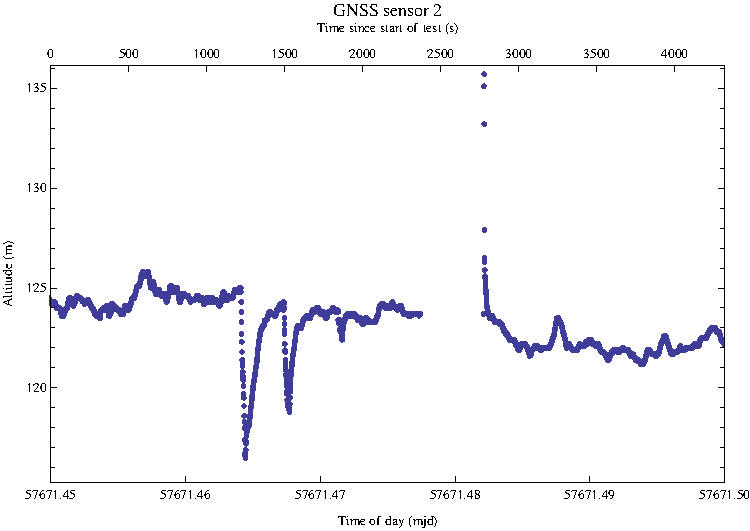
\includegraphics[width=1\textwidth]{gnssAlt2.pdf}
  \caption{The figure shows the solved altitude of the GPS receiver connected to Sensor 2, during test 1}
  \label{sensor2_alt}
\end{figure}

\begin{figure}
  \centering
  \includegraphics[width=1\textwidth]{gnssLat1.pdf}
  \caption{The figure shows the solved latitude of the GPS receiver connected to Sensor 1, during test 1}
  \label{sensor1_lat}
\end{figure} 

\begin{figure}
  \centering
  \includegraphics[width=1\textwidth]{gnssLat2.pdf}
  \caption{The figure shows the solved latitude of the GPS receiver connected to Sensor 2, during test 1}
  \label{sensor2_lat}
\end{figure} 

\begin{figure}
  \centering
  \includegraphics[width=1\textwidth]{gnssLong1.pdf}
  \caption{The figure shows the solved longitude of the GPS receiver connected to Sensor 1, during test 1}
  \label{sensor1_long}
\end{figure} 

\begin{figure}
  \centering
  \includegraphics[width=1\textwidth]{gnssLong2.pdf}
  \caption{The figure shows the solved longitude of the GPS receiver connected to Sensor 2, during test 1}
  \label{sensor2_long}
\end{figure} 

\begin{figure}
  \centering
  \includegraphics[width=1\textwidth]{gnssSpeed1.pdf}
  \caption{The figure shows the solved speed of the GPS receiver connected to Sensor 1, during test 1}
  \label{sensor1_speed}
\end{figure} 

\begin{figure}
  \centering
  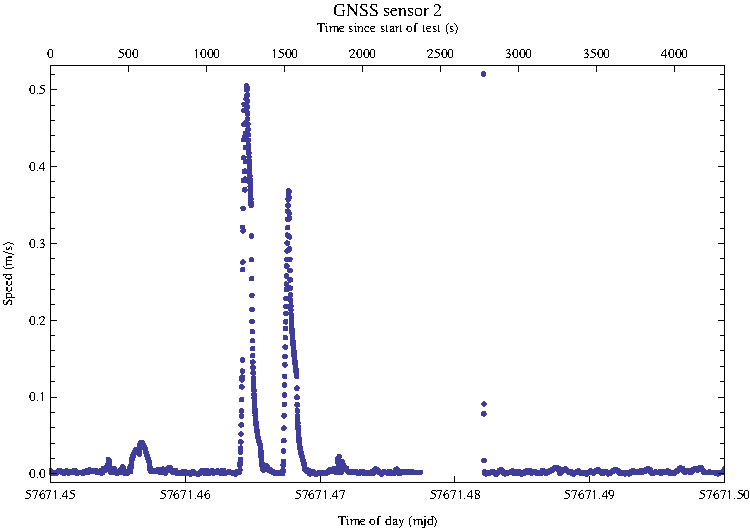
\includegraphics[width=1\textwidth]{gnssSpeed2.pdf}
  \caption{The figure shows the solved speed of the GPS receiver connected to Sensor 2, during test 1}
  \label{sensor2_speed}
\end{figure} 

\newpage
\subsection{Measurements}
Figure \ref{cns91_tel_freq} shows the relative frequency offset($10^{12}$) for the atomic clock. The thick dark plot in the middle is from telemetry data gathered from the atomic clock. Figure \ref{cns91_tel_phase} shows the phase offset in nano seconds for the atomic clock. The interesting thing to observe in both of these figures, is the jump in frequency and phase offset once the antenna was covered in foil. There is also a clear correlation between movement of the antenna and the relative frequency offset as seen in figure \ref{cns91_tel_freq}. 

\begin{figure}[!htb]
  \centering
  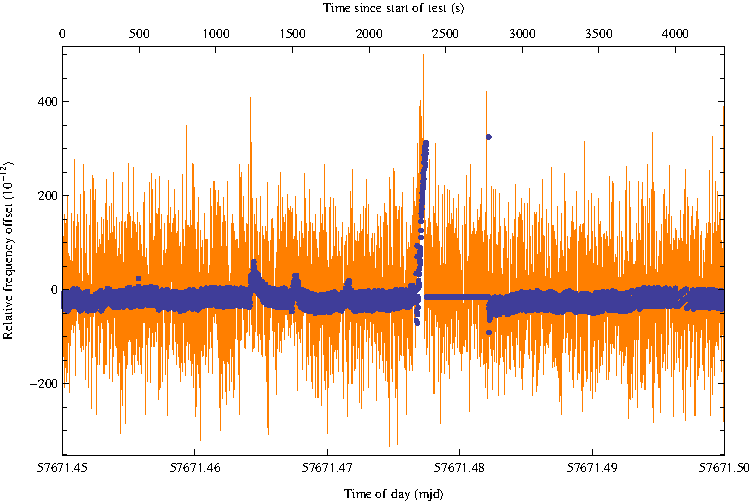
\includegraphics[width=1\textwidth]{cns91-and-csac-telemetry-frequency.pdf}
  \caption{The figure shows the relative frequency offset for the atomic clock. The thick dark plot in the middle is from telemetry data gathered from the atomic clock. The lighter plot in the background is data from the CNT-91 frequency counter.}
  \label{cns91_tel_freq}
\end{figure} 

\begin{figure}
  \centering
  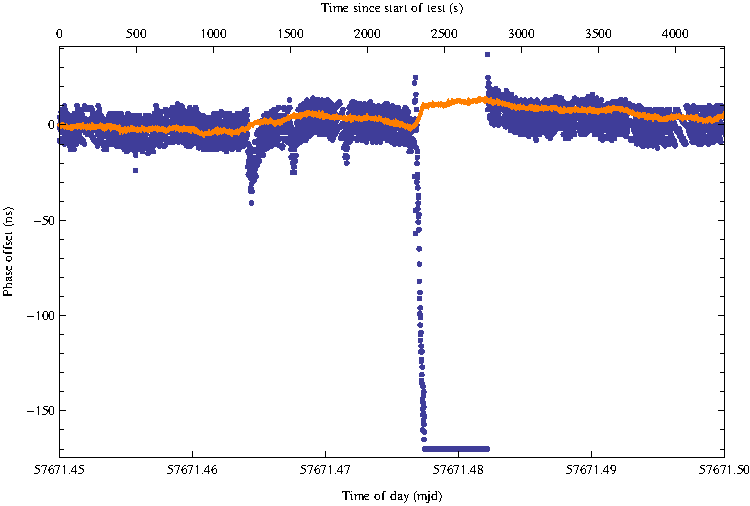
\includegraphics[width=1\textwidth]{cns91-and-csac-telemetry-phase.pdf}
  \caption{The figure shows the phase offset in nano seconds for the atomic clock. The thick dark plot is from telemetry data gathered from the atomic clock. The lighter thin plot is data from the CNT-91 frequency counter.}
  \label{cns91_tel_phase}
\end{figure} 

\subsection{Conclusion}
The observations reveal what we expected. After all, when moving a GPS receivers antenna, the solved position has to change. If it did not, the GPS receiver or antenna would have to be faulty. Step 5 and 6 did not produce the expected result. The reason was discovered to be an error in the KRL filter configuration. One of the clock model based filters where also triggered, which we did not expect. The filter that was triggered was the \textit{Simple prediction filter}. See \ref{csac_filters} for more about the clock model based filters. 

\newpage
\section{Test 2}
\subsection{Goal of test}
The goal of the second test was to reproduce the result from test 1, where one of the clock model based filters were triggered. This should make the Sensor Server disable the atomic clock's disciplining mode and steer the atomic clock after the clock model's predictions. We also wanted to test the KRL filter again to make sure we had fixed the error in the filter's configuration, from last test.

\subsection{Change in setup}
The setup in test 1 is quite similar to test 2. There is however some changes. Sensor 1 is no longer connected to the Sensor Server since the KRL filter no longer was main priority. Sensor 2 did however still log data during the test as it did during test 1.

\subsection{Description}\label{test2_description}
The description of test 2 is similar to test 1(\ref{test1_description}). The only difference is that greater care was taken in obtaining an accurate time for the steps.

\begin{itemize}
  \item\relax 13:12:00 - 125: Started to move antenna 2 towards north.
  \item\relax 13:12:45 - 170: Reached destination.
  \item\relax 13:18:00 - 485: Started the move back to original location.
  \item\relax 13:19:00 - 545: Reached destination.
  \item\relax 13:23:00 - 785: Waved the antenna around at an increasing tempo in a half circle motion.
  \item\relax 13:23:45 - 830: Stopped waving.
  \item\relax 13:27:00 - 1070: Manually enabled the disciplining of the atomic clock.
\end{itemize}

\subsection{Observations}\label{test2_observations}
\subsubsection{Sensor Server logs}
The following By reviewing the log produced by the Sensor Server, the following was observed:

\begin{itemize}
  \item No false positives, the filters were not triggered before the test started.
  \item The KRL filter was triggered by at 13:12:10 and cleared at 13:19:54
  \begin{lstlisting}
    [10/24/16 - 13:12:10] [ ALARM ] Sensor 2 triggered KRL filter!
    ...
    [10/24/16 - 13:19:54] [ ALARM ] Sensor 2 cleared KRL filter!
  \end{lstlisting}
  \item The KRL filter was triggered again at 13:23:12 for only a second. It was then triggered again two seconds later and was not cleared 13:23:43.
    \begin{lstlisting}
    [10/24/16 - 13:23:12] [ ALARM ] Sensor 2 triggered KRL filter!
    ...
    [10/24/16 - 13:23:13] [ ALARM ] Sensor 2 cleared KRL filter!
    ...
    [10/24/16 - 13:23:15] [ ALARM ] Sensor 2 triggered KRL filter!
    ...
    [10/24/16 - 13:23:43] [ ALARM ] Sensor 2 cleared KRL filter!
  \end{lstlisting}
  \item More interestingly was the fact the \textit{Frequency correction filter} was triggered. This is what we wanted. 
    \begin{lstlisting}
      [10/24/16 - 13:12:42] [ ALARM ] Steer > predicted!
    \end{lstlisting}
\end{itemize}

\subsubsection{GPS data}
Figure \ref{sensor2_everything} shows the plotted GPS data collected during test 2. As with GPS observed during test 1, there is a clear correlation between the plotted data and when the antenna was moved. The strange phenomena as described in test 1 (\ref{gpsdata_test1}) where the altitude was reported to be way too low, occurred in test 2 as well. 

\begin{figure}
  \centering
  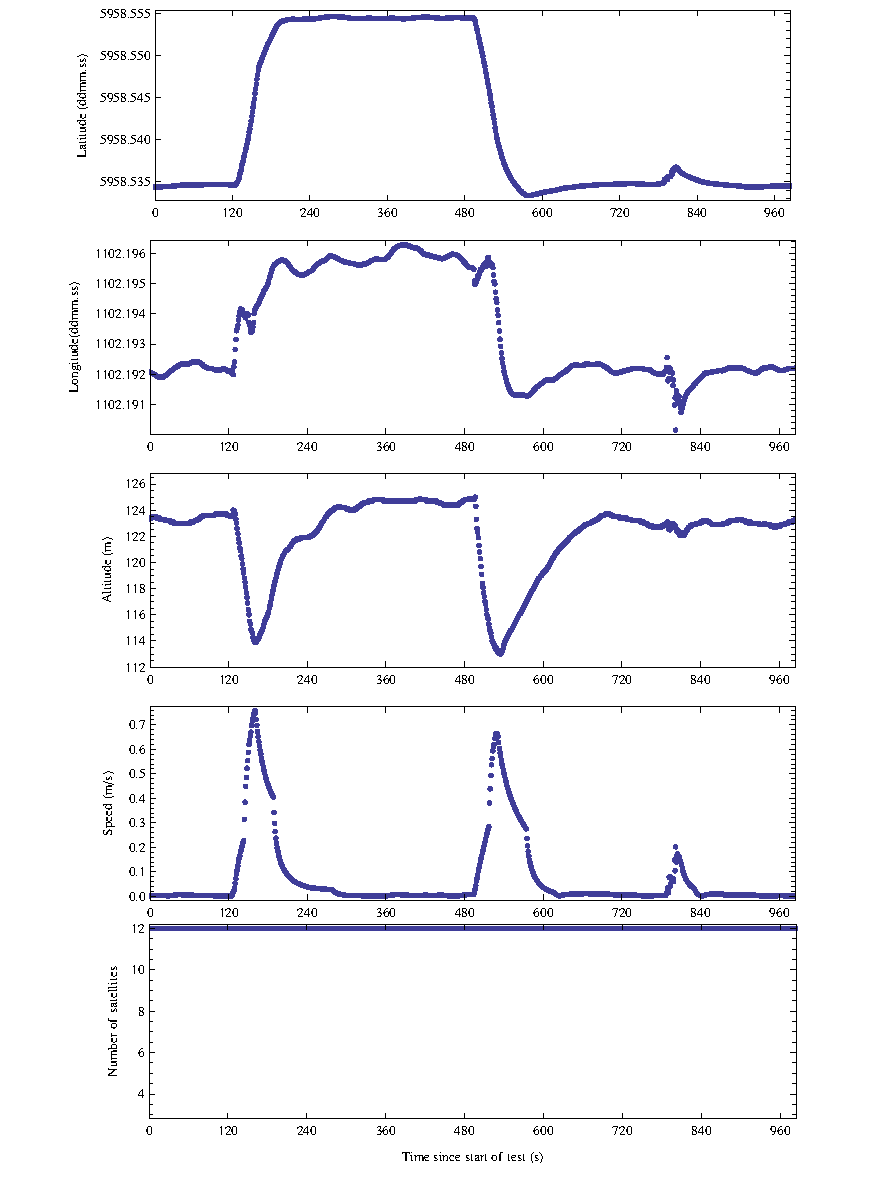
\includegraphics[width=1\textwidth]{20161024-test2-sensor2-multipanel.pdf}
  \caption{The figure shows (from the top) the latitude, longitude, altitude, speed and number of satellites as plotted from the GPS data collected during test 2.}
  \label{sensor2_everything}
\end{figure} 

\newpage
\subsection{Measurements}

\begin{figure}
  \centering
  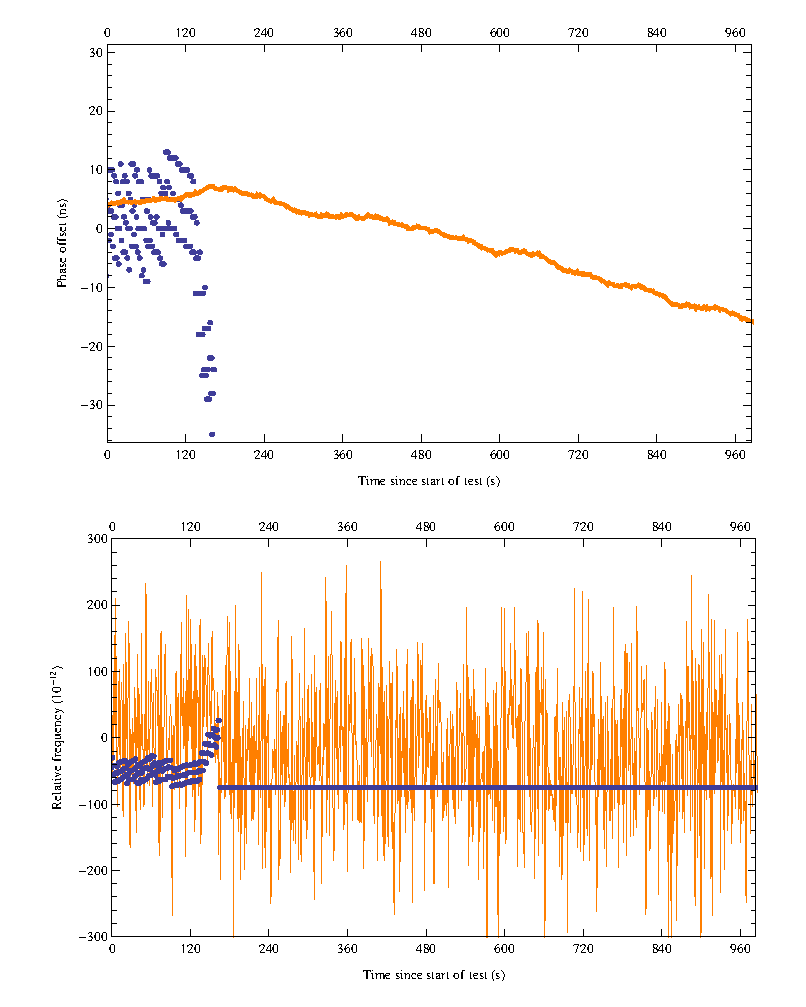
\includegraphics[width=1\textwidth]{20161024-test2-telemetry-and-cnt91-combined.pdf.pdf}
  \caption{The figure shows (from the top) the latitude, longitude, altitude, speed and number of satellites as plotted from the GPS data collected during test 2.}
  \label{sensor2_everything}
\end{figure} 

\subsection{Conclusion}
Disabling of disciplining worked fine. The steering did not.

